\documentclass[12pt]{article}

\pdfminorversion=4

\usepackage[utf8]{inputenc} %unicode support

\usepackage{amsmath}
\usepackage{amssymb}
%\usepackage{pdfpages}
\usepackage{gensymb}
\usepackage{graphicx}
\usepackage{epstopdf}
\usepackage{color}
\usepackage[margin=1in]{geometry}
\usepackage{times,mathptmx}

% Bold the 'Figure #' in the caption and separate it with a period
% Captions will be left justified
\usepackage[labelfont=bf,labelsep=period,justification=raggedright]{caption}

% Use the ACS provided bibtex style
%\bibliographystyle{plain}
\bibliographystyle{acs}
\usepackage{cite}

% Remove brackets from numbering in List of References
\makeatletter
\renewcommand{\@biblabel}[1]{\quad#1.}
\makeatother


% definition of \customlabel, which is used to label supplementary figures and tables
\makeatletter
\newcommand{\customlabel}[2]{%
\protected@write \@auxout {}{\string \newlabel {#1}{{#2}{}}}}
\makeatother


\begin{document}


\title{Large-scale analysis of post-translational modifications in \emph{E. coli} under glucose-limiting conditions over 2 weeks}

\author{Viswanadham Sridhara$^1$, Daniel R. Boutz$^{2,3}$, Craig Barnhart$^3$, Jeffrey E. Barrick$^{1,2,3,4}$,\\
Edward M. Marcotte$^{1,2,3,4,5}$, and Claus O. Wilke$^{1,2,3,5}$}
\maketitle

\noindent
$^1$Center for Computational Biology and Bioinformatics, The University of Texas at Austin, Austin, TX, USA\\
$^2$Institute for Cellular and Molecular Biology, The University of Texas at Austin, Austin, TX, USA\\
$^3$Center for Systems and Synthetic Biology, The University of Texas at Austin, Austin, TX, USA\\
$^4$Department of Molecular Biosciences, The University of Texas at Austin, Austin, TX, USA\\
$^5$Department of Integrative Biology, The University of Texas at Austin, Austin, TX, USA\\


\begin{abstract}
A 
\end{abstract}

% keywords: post-translational modifications

\section{Introduction}

Most of the times, specific biological function of the proteins is identified by the post-translational modification associated with it. Much work has been done in identifying the protein coding genes, however, identification of the functional PTMs is still at its infancy. Mass-spectrometry (MS) based proteomics is the only technique that can characterize these PTMs in large scale. Peptide search algorithms are then run on these mass-spectrometry data sets to identify peptides and PTMs associated with it. Here we used MS on E. coli proteome grown under glucose-limiting conditions and then identified various PTMs in large scale.

Identifying a targeted list of PTMs (mostly up to 6) is a general norm with most of the sequence search algorithms. As the number of target PTMs increase, search space and the false positives generally increase that limits the number of input PTMs. However recently, software for unrestricted search of PTMs is starting to grow. We used MODa, a naive based multi-blind spectral alignment algorithm, to look for PTMs in this dataset. 

Most of the studies till date limit to capturing RNA/proteome information to 1 or 2 time points during exponential and stationary phases for analysis. Here we collected MS data on E. coli proteome at 9 different time points ranging from exponential to long-stationary phases up to 2 weeks under glucose-limiting conditions. To our knowledge this is a first attempt to look into time-course of PTMs over 2 weeks of a microbe.

\cite{Stadtman1992}
{Protein oxidation and aging}

\cite{Vogt1995}
{Oxidation of methionyl residues in proteins: tools, targets, and reversal}

\cite{Grimaudetal2001}
{Repair of oxidized proteins. Identification of a new methionine sulfoxide reductase},

\cite{Tete-Favieretal2000}
{Crystal structure of the Escherichia coli peptide methionine sulphoxide reductase at 1.9 A resolution}
   
\cite{Tete-Favieretal2000b}
{Crystallization and preliminary X-ray diffraction studies of the peptide methionine sulfoxide reductase from Escherichia coli}
   
\cite{ZhangWeissbach2008}
{Origin and evolution of the protein-repairing enzymes methionine sulphoxide reductases}
   
This fixation of MsrA is helpful \cite{Abramsetal1981}
{Enzymatic reduction of oxidized alpha-1-proteinase inhibitor restores biological activity}

\cite{Davisetal2000}
{HIV-2 protease is inactivated after oxidation at the dimer interface and activity can be partly restored with methionine sulphoxide reductase}

Mascot\cite{Perkinsetal1999}, Sequest \cite{Engetal1994}, OMSSA \cite{Geeretal2004}, X!Tandem \cite{CraigBeavis2004}, TagRecon\cite{Dasarietal2010}, MODa\cite{Naetal2012}, and Byonic \cite{Bernetal2012}

Large-scale analysis of PTMs \cite{OlsenMann2013}

PTM network motif \cite{Olsenetal2006}
{Global, in vivo, and site-specific phosphorylation dynamics in signaling networks}

PTM cross talk \cite{Pengetal2014}
{Identification of enriched PTM crosstalk motifs from large-scale experimental data sets}

\cite{Charbautetal2002}
{N-terminal acetylation of ectopic recombinant proteins in Escherichia coli}

Msr fixing MetSO to Met \cite{Brotetal1981}
{Enzymatic reduction of protein-bound methionine sulfoxide}

\cite{Ezratyetal2004}
{Methionine sulfoxide reductases protect Ffh from oxidative damages in Escherichia coli}

\cite{Driessenetal1985}
{The mechanism of N-terminal acetylation of proteins}

\cite{Helbigetal2010}
{Profiling of N-acetylated protein termini provides in-depth insights into the N-terminal nature of the proteome},

\cite{Gordiyenkoetal2008}
 {Acetylation of L12 increases interactions in the Escherichia coli ribosomal stalk complex}
 
\cite{Polevodaetal2003}
{Nat3p and Mdm20p are required for function of yeast NatB Nalpha-terminal acetyltransferase and of actin and tropomyosin}
   
\cite{PolevodaSherman2003}
{Composition and function of the eukaryotic N-terminal acetyltransferase subunits},
   
\cite{PolevodaSherman2003b}
{N-terminal acetyltransferases and sequence requirements for N-terminal acetylation of eukaryotic proteins}

\cite{Starheimetal2012}
{Protein N-terminal acetyltransferases: when the start matters}

\cite{Tanakaetal1989}
{Cloning and molecular characterization of the gene rimL which encodes an enzyme acetylating ribosomal protein L12 of Escherichia coli K12}

\cite{Yoshikawaetal1987}
{Cloning and nucleotide sequencing of the genes rimI and rimJ which encode enzymes acetylating ribosomal proteins S18 and S5 of Escherichia coli K12}
   
MODa application \cite{Kimetal2014}
{ROSics: Chemistry and proteomics of cysteine modifications in redox biology}

N-terminal processing \cite{Kimuraetal2003}
{N-Terminal modifications of the 19S regulatory particle subunits of the yeast proteasome}

Mass-spec E. coli proteome \cite{Krugetal2013}
{Deep coverage of the Escherichia coli proteome enables the assessment of false discovery rates in simple proteogenomic experiments},

MODa application in urine proteomics \cite{Liuetal2013}
{Unrestrictive identification of post-translational modifications in the urine proteome without enrichment},

E. coli phosphoproteomics \cite{Maceketal2008}
{Phosphoproteome analysis of E. coli reveals evolutionary conservation of bacterial Ser/Thr/Tyr phosphorylation}

E. coli phosphoproteome dynamics \cite{Soaresetal2013}
{Global dynamics of the Escherichia coli proteome and phosphoproteome during growth in minimal medium},

E. coli nitrosylation \cite{Sethetal2012}
{Endogenous protein S-Nitrosylation in E. coli: regulation by OxyR},


Research into 

\section{Results}

We wanted to use an unrestricted approach to find the post-translational modifications in E. coli sample grown under glucose-limited conditions. This sample is not enriched for any post-translational modifications. So, the coverage of the PTMs identified is limited, however we can get information on most of the PTMs.
 
\subsection{Running MODa on \emph{E. coli} proteome}
We did this analysis using MODa, a naive based spectral alignment search algorithm. Unlike other peptide identification search algorithms, MODa requires as an input the range of PTM masses instead of the actual PTMs. So, for our analysis we used a range of -200 to 200 Da which is typical to this search engine. We generated mass-spec raw data at different time points in exponential and stationary phases of E. coli growth.
At each of the 9 time points, we have 3 biological replicates. For each of the replicates, we ran MODa. We asked some of the following questions while analyzing the data:
(a) How much of the proteome is modified? (b) How do these modifications change over time? (c) Can we find any novel modifications? (d) Can we explain the pattern of the PTMs over time using other diverse kinds of data such as RNA-seq?

\subsection{Modified \emph{E. coli} proteome}
To estimate how much of the proteome is modified, we counted the number of peptide-spectral matches (PSMs) for each MODa run. We used standard error to plot the variation within 3 biological replicates.
Figure 1 shows the total percent of the peptide-spectral matches on the y-axis and the growth curve time on the x-axis. Consistently 25\% of the peptide-spectral matches seem to be modified at all the 9 time points analyzed.
This is in agreement with some of the previous studies (Cite papers which show the same numbers). However note that a modification could be a mutation or a post-translational modification.

\subsection{N-term protein acetylations are frequent in \emph{E. coli}}
Since MODa outputs mass-shift, we used UNIMOD database to map the mass-shift to the probable PTM. MODa outputs not only the mass-shifts, but also the amino-acids on which this mass-shift occurs. We focussed not only on the most common PTM-amino acid combination, but also on the PTMs irrespective of the amino acid. For example, we know acetylation is most common on n-term and lysine, however we also looked at the time-course of all acetylations i.e., sum of acetylations on all amino acids. (Add other citations and results from literature)

\subsection{\emph{E. coli} carboxylations, nitrosylations and other PTMs}
To understand what kinds of PTMs or mutations are present in the sample, we plotted the frequency of the mass-shifts from the MODa output. MODa program calculates the mass-shifts in intervals of 1Da, along with the amino acid on which it finds the mass-shift. Along with the amino acids, it also calculates the N-term and C-term mass-shifts. Figure 2 shows the mass-shift frequency matrix. A zoomed-in version (b) shows that +1 Da peak is the most frequent one. However this modification seems to be 13C peak-picking as it seems to occur on all the amino acids, when we looked at the profile (Suppl Figure 1). Next frequent modification is +16Da. A look at profile (Suppl Figure 2) shows majority of oxidations on methionine which is expected.

Next we looked at the time course evolution of few post-translational modifications. In particular, we looked at acetylations, carboxylations, nitrosylations, phosphorylations and oxidiations. Figure 3 shows the time course evolution of all acetylations, along with N-term and serine acetylations which seem the dominant ones. A close look at the serine acetylations show that they fall at the N-term x\% of the time. During the exponential phase, the acetylations seem not to change much over time. However during the stationary and the long-stationary phases, the acetylations seem to go up. E. coli grown on glucose have shown to accumulate acetate (Cite proper references). Our results might suggest the same given the increase in the number of acetylated proteins from exponential to stationary phases. Table 1 shows the acetylated proteins found under these 2 different phases under E. coli growth under glucose limiting conditions.

Next, we investigated the phosphorylations found in this study. Note that this study is not enriched for phosphorylation or other modifications. Typically studies that identify phosphopeptides are generally enriched for phosphorylations using IMAC or TiO2. However as we mentioned early, our goal is to identify different kinds of PTMs in this proteomics data. Figure 4 shows the phosphorylations at different points of the growth curve. The number of phosphorylations seem to be small and there is an increase of the number of phosphorylations from exponential to stationary phases. Similarly we looked at the carboxylations and nitrosylations (Suppl Figure 3), as they are shown in the past to be important in E. coli. Suppl Figure 4 shows the Na and K adduct profiles. They seem to occur on all the amino acids, except basic charge amino acids.

Pyroglutamate conversion and Succinylation:
Glutamine conversion at n-term of the peptide to pyroglutamate is a well known PTM. Suppl Figure 5 shows that this conversion seems to be more or less same at different phases of the growth. (Add data about succinylation)

\subsection{Oxidative damage and repair in \emph{E. coli}}
Finally, we investigated oxidative damage by looking at the oxidations identified by MODa program i.e.., mass-shifts of +16Da. The oxidations seem to go down from exponential to stationary phases. This result seemed strange as we expected oxidative damage and hence the oxidations to go up as the E. coli reaches stationary and long-stationary phases. However may be the sulfoxide reductases MsrA and MsrB found in e. coli seem to fix methionine sulfoxide back to methionine. Since we also gather RNA-seq data on the same sample, we were able to retrieve the transcriptomic abundances of MsrA and MsrB along with proteomic abundances. There is not much change in the profiles of transcripts of these reductases i.e., the abundance seem to go down from exponential to stationary and stayed flat during long stationary phase. However the proteomic abundance seem to go down initially from exponential to stationary phase, however it surged up during the long-stationary phase indicating the probable fixing of MetSO to Met. Previously it was shown that these reductases play a role, however in this study for the first time we showed the time course fixation of MetSO to Met.

%Comparison with Sequest on methionine oxidations:
%We also did Sequest searches but only with methionine oxidation as variable modification. We compared the number of oxidations on methionine in MODa and Sequest and also plotted the time course of these oxidations at different phases of the E. coli growth curve under glucose-limiting conditions. (Add results here)


\subsection{Novel phosphoserinegluconylation on ribosomal protein S6}
To see if the results and trends of the PTMs over time holds, we changed the MODa range search from -300 to 300Da. The trends and the results were the same as previously shown. However, a +258 Da shift on serine is found consistently at all time points of the growth curve. When we looked into into literature, this seemed to be a phosphorylation+gluconylation on Serine, which is a known modification. However it was not shown in literature to occur frequently on the ribosomal protein S6 in E. coli.

\subsection{ in \emph{E. coli}}

\section{Discussion}

Limitations:
Large-scale PTM analysis is still at its infancy because of both experimental enrichment techniques of PTMs as well as the computational search algorithms that have to look at different combinations to identify the PTMs. Here we used MODa, a naive based search algorithm on E. coli proteome data obtained under glucose-limiting conditions. Our analysis showed that 1/3rd of the peptide spectral matches found are modified. We also saw a decrease in oxidation levels from exponential to stationary phase, with sulfoxide reductases playing a role in fixing Methionine oxide back to methionine. n-term acetylations are frequent, with serine n-term acetylation happening 75\% of all n-term acetylations, all the times on the 2nd amino acids of the protein, after methionine excision. Phosphorylation increased from exponential to stationary phases, while carboxylations and nitrosylations remained constant throughout the time course of E. coli growth. Na and K adducts seem to happen 3-4\% of the time. Finally, a novel serine modification i.e., phosphogluocnylation of serine seems to happen on ribosomal protein S6 frequently.

Most of the peptide identification search algorithms required a list of PTMs to search for and usually this list is limited to 6. However databases like UNIMOD, RESID have listed at least 400 known PTMs present. So, we used a naive based search algorithm that outputs mass-shifts, instead of the PTMs in the peptide-spectral match. Then we use UNIMOD to identify the PTM that matches the mass-shift. However we did not try and match all the mass-shifts, but investigated in detail the frequent mass-shifts identified by MODa. One limitation is we used the default mass-range search between -200 and 200 Da and one other search with -100 and 300 Da range. So, we miss out on larger PTMs i.e., polyubiquitination tails etc. This resulted in analysis of +1 Da mass-shift (C13 peak detection), oxidation, acetylation, Na and K adducts, along with some widely studied PTMs in phosphorylation, carboxylation and nitrosylation. This program is previously used for similar large-scale analysis with urinary proteomics and they identified novel PTMs. However the study used 2 programs and considered the overlap of PTMs as highly confident. Instead here, our focus is not to identify highly-confident PTMs later used as biomarkers, but to get a wider coverage at a lower FDR of 1\% and look at the time course or evolution of these PTMs during the entire 2 weeks of E. coli growth.

To avoid false positives and as recommended by the original MODa paper, we ran search engine looking for only 1 possible modification on the peptide. Generally the PTMs are validated by a 2nd round of identifying highly confident hits. This is usually done by using programs like Ascore etc. However here, we did not do any 2nd round of validating peptides. Also, we looked at the global level of PTMs, instead of counting which peptide and hence protein is modified. We did not do any PTM level quantitation or try to undestand the specific PTM stoichiometry, as these require sophisticated experimental instrumentation, protocol and the algorithms to characterize the PTMs associated with proteins.

Nice review article on E. coli proteomics by different technologies including MS can be found here:
Cite this paper: The Escherichia coli Proteome: Past, Present, and Future Prospects†
Mee-Jung Han1 and Sang Yup Lee1,2,*

Directly taken from the above paper for my future analyses: For example, SspA expression increased with decreasing growth rate and was induced by glucose, nitrogen, phosphate, or amino acid starvation. Furthermore, the proteome profiles during the exponential growth phase showed that the expression levels of at least 11 proteins were altered in sspA mutant strains (314). These findings indicate that SspA acts as a transcription factor and is essential for starvation stress-induced tolerance (e.g., stationary phase) in E. coli.

Copied from the same paper At the onset of glucose starvation, cyclic AMP and its receptor protein (cAMP-CRP) were found to play important roles in the expression of a number of genes. An early 2-DE study identified five glucose-responsive outer membrane proteins (four upregulated and one downregulated) (186). A comparison with membrane proteins from mutant strains revealed that two of the upregulated proteins were the receptors for lambda and T6, and coelectrophoresis of the outer membrane fraction identified the downregulated protein as OmpA. The glucose starvation stimulon was further examined using 2-DE followed by comparison to the E. coli gene-protein database (218). Members of this stimulon were found to include enzymes of the Embden-Meyerhof-Parnas pathway, phosphotransacetylase (Pta) and acetate kinase (AckA) in the acetic acid pathway, and formate transacetylase. Trichloroacetic acid cycle enzymes were repressed, whereas enzymes involved in acetate and formate production and the Embden-Meyerhof-Parnas pathway were induced. These modulations suggest that a glucose-starved cell increases the relative flow of carbon through the Pta-AckA pathway. Indeed, pta and pta-ackA mutants were found to be impaired in their abilities to survive glucose starvation, indicating that the capacity to synthesize acetyl phosphate, an intermediate of this pathway, is indispensable for glucose-starved cells. The pta mutant failed to induce several proteins of the glucose starvation stimulon. More recently, proteome studies revealed that glucose limitation upregulates the levels of proteins such as AceA, AldA, ArgT, AtpA, DppA, GatY, LivJ, MalE, MglB, RbsB, UgpB, and YdcS (311). Of these, ArgT, DppA, LivJ, MalE, MglB, RbsB, UgpB, and YdcS are periplasmic binding proteins of the ABC transporters, suggesting that in addition to the central metabolism proteins, periplasmic binding proteins are involved in the carbohydrate and amino acid uptakes that are important during glucose limitation.

Also, A functional relA gene is required for sspA to affect protein synthesis. (taken from another paper)
Interesting to find PTMs on these proteins?

Total proteins could be the same - should I plot the total number of proteins over time? absolute protein abundances calculated from APEX protocol?

Most of the times, proteins act in complexes to perform a specific function. In such process, 1 or few amino acids of a protein interact with other residues of another protein, generally through the PTMs. So, large-scale analysis of PTMs such as this work would help us better understand the fine granularity at PTM level that is responsible for a particular mechanism, such as multiple phosphorylations in the case of signalling cascades.

Mass-spec analysis of human soluble protein complexes has revealed a large number of conserved complexes along with thousands of protein-protein interactions. Large-scale analysis of PTMs on these kinds of proteomics data would help to understand these interactions at PTM level. Such annotations could then be integrated with databases such as NCBI CDD
Across diverse species (cite Emili/Marcotte collaboration cell papers) and talk about PTM annotation in databases like CDD? Cite the paper on conservation of phosphorylations etc on CDDs, but extend to other PTMs?

Current whole-cell models \cite{Covertetal2008} are trying to integrate diverse kinds of OMICS data i.e., transcriptomics, proteomics not only to refine the existing models but also get the response of the models close to the experimental metabolic flux measurements. Here, we argue that including the modification information (i.e., number of modified proteins to that of the unmodified version) will improve the existing methodologies.



\section{Conclusions}

We have found


\section{Materials and Methods}

\subsection{\emph{E. coli} growth} 
Craig Barnhart part (Copied from John’s paper):
E. coli B REL606 was inoculated from freezer stock in 50mL DM500 and incubated at 37C overnight. 500 UL \emph{change to micro} of the overnight culture was diluted in 50mL of DM500 at 37C and grown for 24hrs. On the day of the experiment, 500 UL \emph{change to micro} of the 24hr culture was added to 10 flasks containing 50mL DM500 each, grown at 37C. At each time point 1ml was removed, washed with 0.7\% NaCl, spun down, the supernatant was removed, and the remaining cell pellet was flash frozen using liquid nitrogen and stored at –80C. Samples for each experiment where taken from the same batch of culture. 

To measure colony forming units (CFU) the OD600, at each time point, was taken relative to sterile DM500 glucose, cultures were diluted in sterile saline, and finally plated on DM agar supplemented with 0.2g/L glucose. Colonies were counted, after incubation at 37C for 24hr. Cultures for measuring CFU were grown separately from the main culture but in identical conditions. 

\subsection{Mass-spectrometry of \emph{E. coli} proteome} 
Dan Boutz part (Copied from John’s paper):
Frozen pellets where re-suspended in 300 uL of buffer (50mM Tris-HCL pH 8.1,100mM KCL, 5mM MgCl2). 50UL of sample was removed for preparation, treated with 50uL trifluoroethanol (TFE), and placed on ice for 15min. DTT was then added to a final concentration of 5mM and incubated at 55C for 45 min. Samples where alkylated by addition of Iodoacetamide (IAM) to a final concentration of 15mM. Trypsin digest was performed by addition of 800uL of 50mM Tris pH 8.0, 2mM CaCl2 followed by 2ug of trypsin. Digestion took place at 37C for 4-5 hrs and was stopped by 10uL of formic acid (1\% vol./vol). Samples where then ultrafiltrated to remove insoluble and undigested material using Amicon Ultra MWCO 10kD spin-caps and finally concentrated and purified by C18 filtration. 
Liquid chormotography and mass spectrometry (LC/MS) was carried out on a LTQ-Orbitrap (Thermo Fisher). <particular settings need to be filled in>

\subsection{Post-translational modification identification and analysis} 
We used MODa (cite) to identify peptides and characterize novel PTMs. MODa outputs mass-shifts on the amino acids instead of the post-translational modifications. So, we used UNIMOD database to map the mass-shift to the appropriate PTM or a mutation. We ran separate searches for each of the 9 time points and at each time point, there were 3 biological replicates. So, there were in total 27 MODa searches. We used TACC for computing resources. The enzyme used in the searches is trypsin with fully-tryptic and no proline rule. The missed cleavages allowed are 2. Since the fragmentation technique used is CID, we looked for b/y ions. The mass-tolerance of the precursor is 10ppm, while the mass-tolerance of the product ion is 0.5 Da. We used carbamidomethylation of cysteine as a static or fixed modification. As mentioned earlier, MODa requires a mass range to search for variable modifications, so we tried 2 scenarios: (a) mass range between -200 to 200Da and (b) second search with mass range between -100 to 300Da. We used REL606 sequence library from NCBI sequence database. To identify high-confidence hits, we used target-decoy approach (cite). In this approach, we reverse the original REL sequences and concatenate to the original sequence database to form a database that is twice as much as of the original sequence database. The idea is that there are as many false positive hits to that of the original database as that of the decoy database. We used a 1\% FDR in this approach which is a general norm in mass-spectrometry based proteomics searches.

(Add how MODa uses score and other features to calculate the probability?), (Also add how MODa can distribute the hits with the charge state?)

\subsection{Raw data and analysis scripts}

All raw data and analysis scripts are available online in the form of a git repository at\\ \texttt{https://github.com/clauswilke/PTMs}.

%\section{Competing interests}
%The authors declare that they have no competing interests.

\section{Author Contributions}
Conceived and designed the experiments: V.S., C.O.W and E.M.M. Performed the experiments: V.S. Analyzed the data: V.S, C.O.W and E.M.M. Wrote the paper: V.S, D.R.B, C.B, J.E.B, C.O.W and E.M.M.

\section{Acknowledgments}
This project was funded by ARO Grant W911NF-12-1-0390. We thank members of the Colin Brown for helpful discussions on post-translational modifications. The Bioinformatics Consulting Group and the Texas Advanced Computing Center (TACC) at UT provided high-performance computing resources. 


%\section{References} (automatically pops up with bibliography)
% Bibliography tex filename
\bibliography{PTMsMODaBibliography}

\newpage

\section*{Figures}

\begin{figure}[!ht]
\centerline{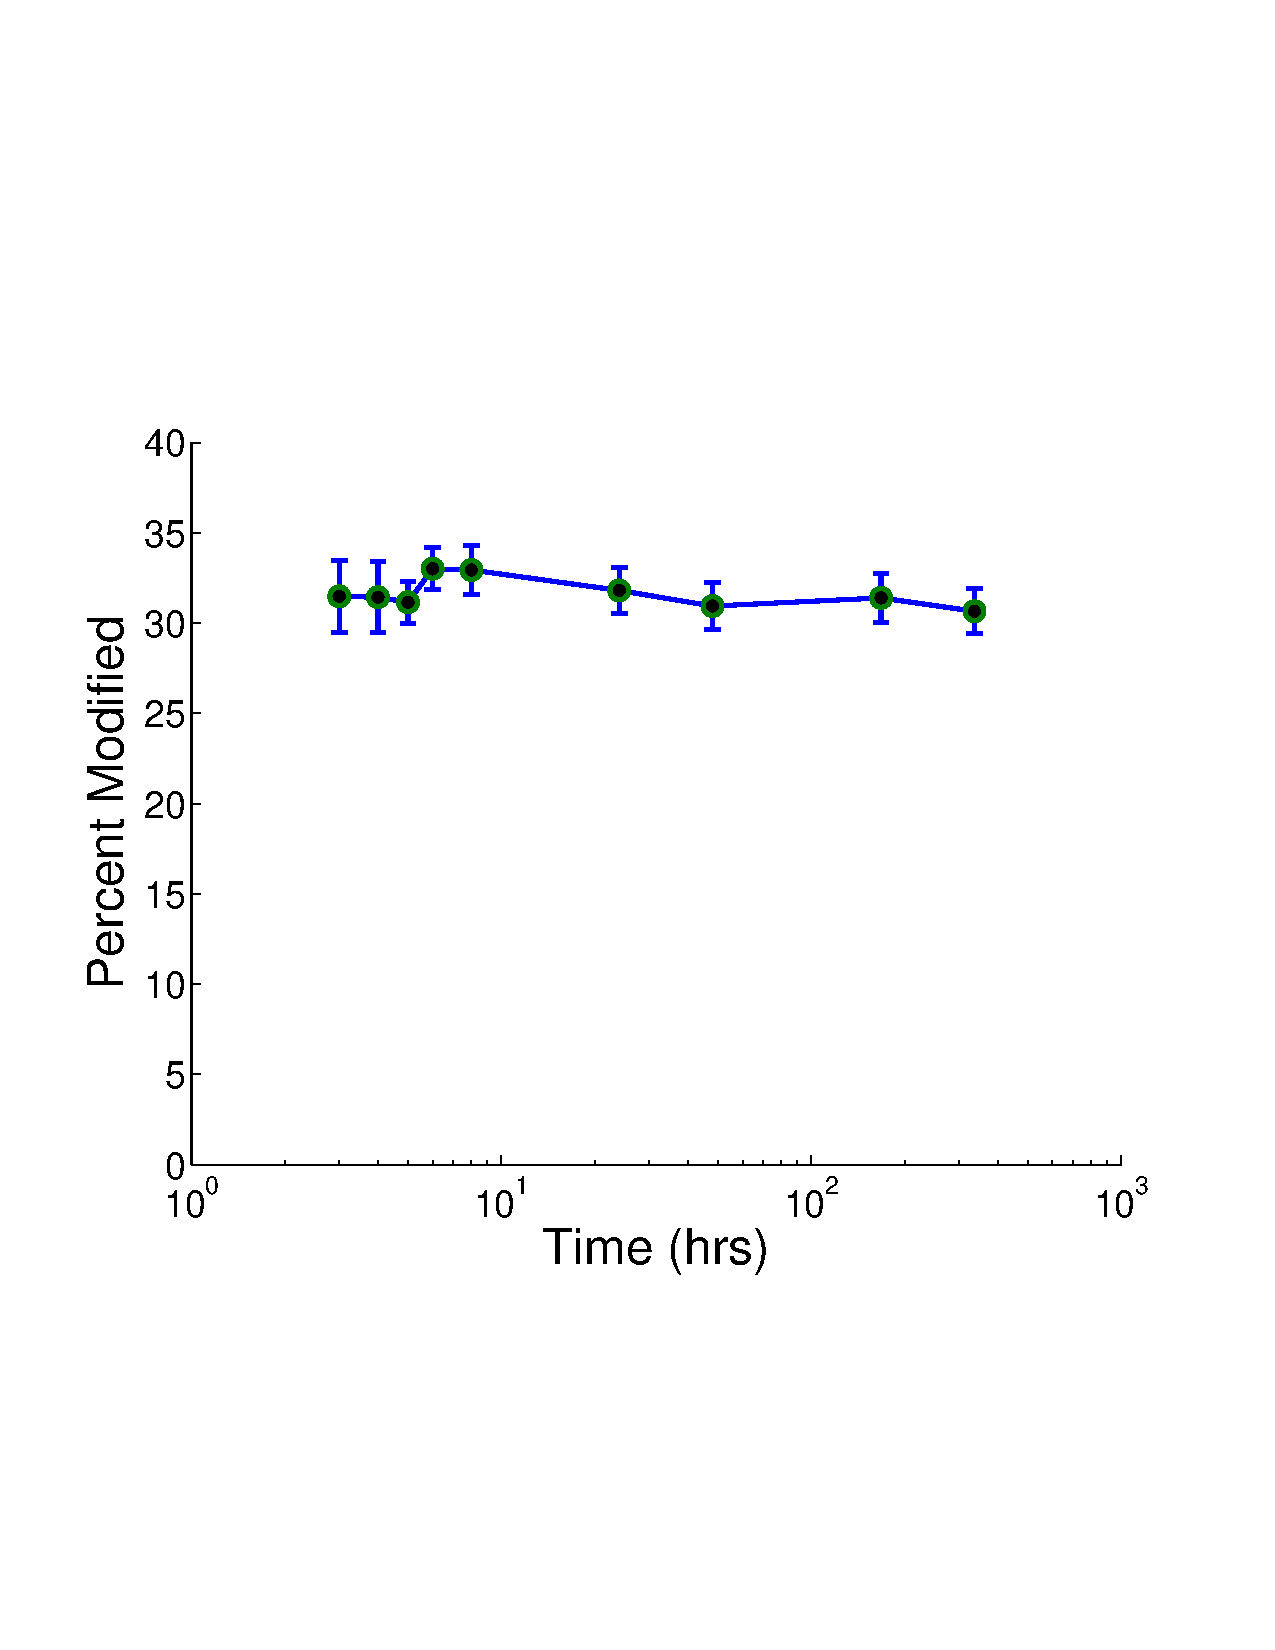
\includegraphics[width=4in]{Figures/Paper_Ecoli_PTM_Modified_Figure1.pdf}}
\caption{\label{fig:flowchart}\textbf{Flowchart.} We use .
}
\end{figure}

\clearpage
\begin{figure}[!ht]
\centerline{\includegraphics[width=8in]{Figures/PTMdalton.pdf}}
\caption{\label{fig:misclassification}\textbf{Misclassification .} For j.}
\end{figure}

\clearpage
\begin{figure}[p]
\centerline{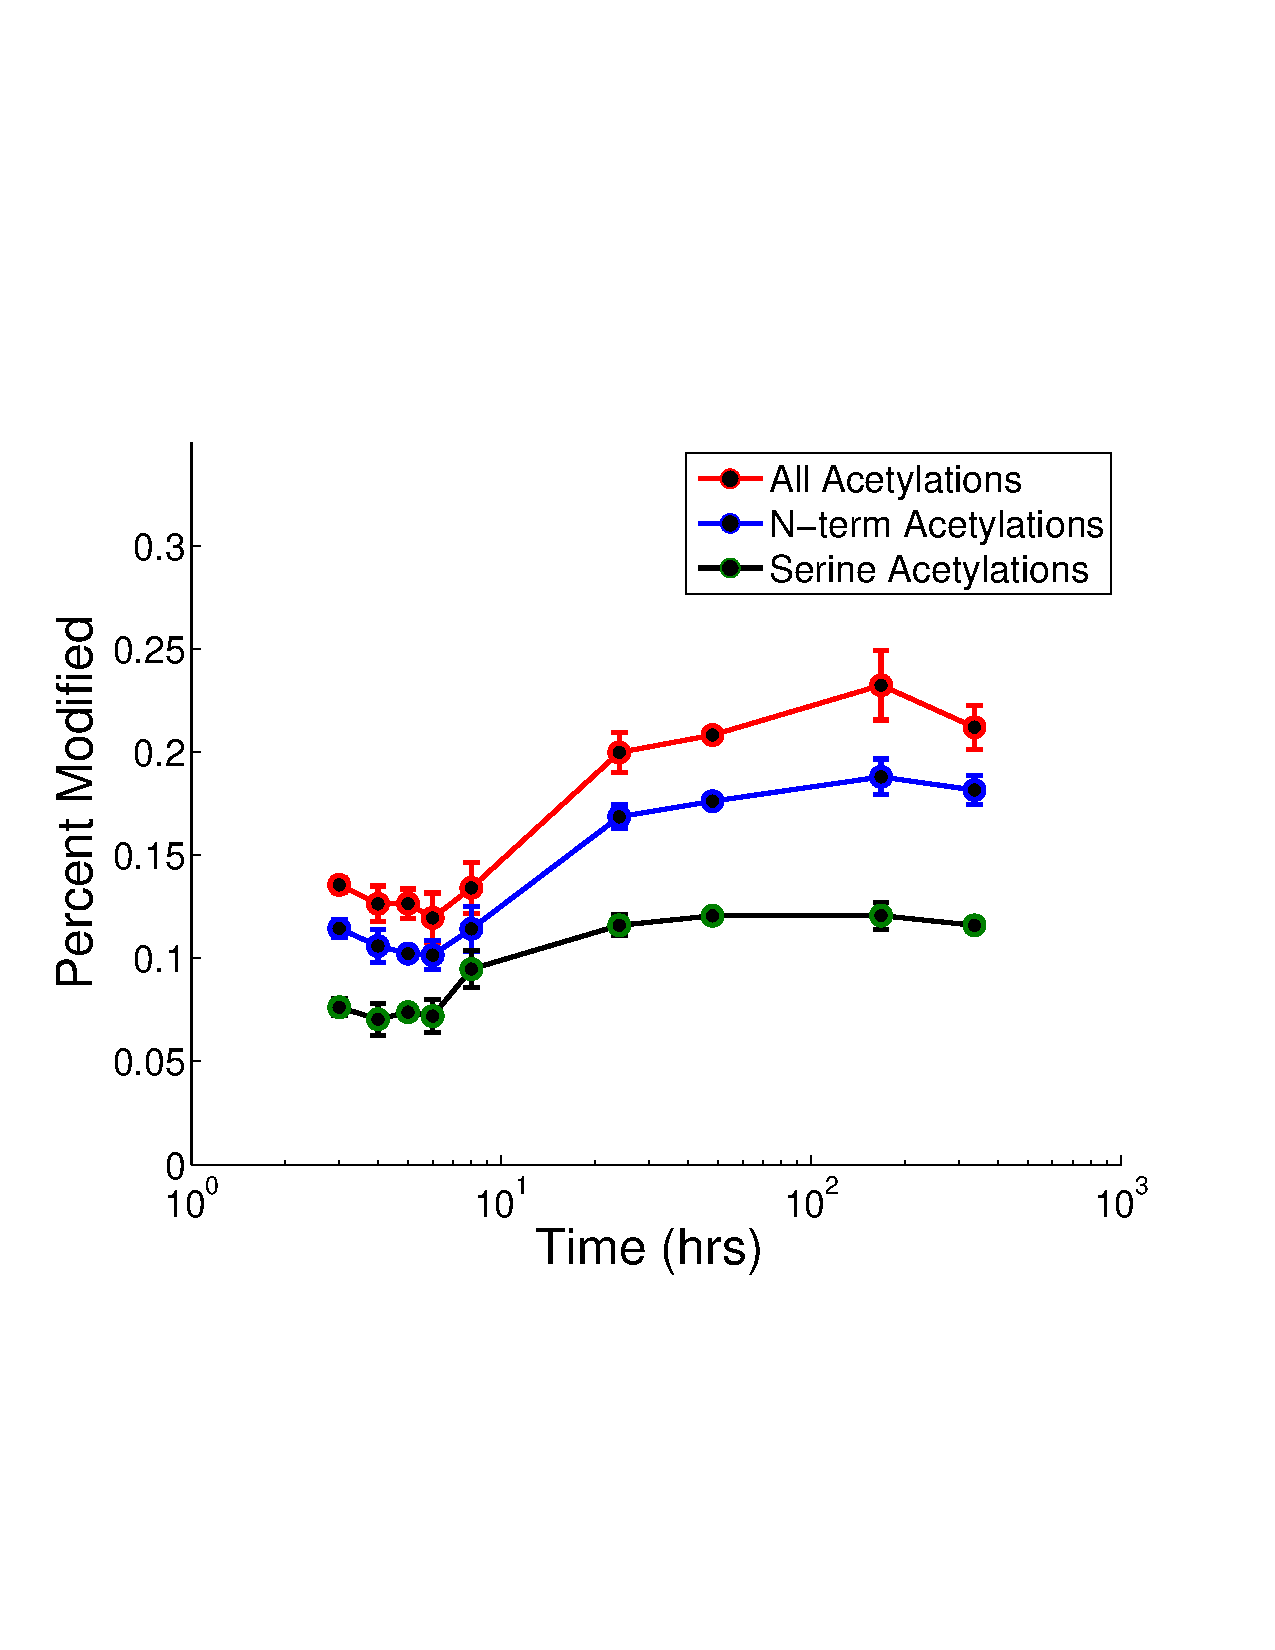
\includegraphics[width=5in]{Figures/Acetylation_AAs.pdf}}
\caption{\label{fig:heat_map}\textbf{Probability .} For .}
\end{figure}

\clearpage
\begin{figure}[p]
\centerline{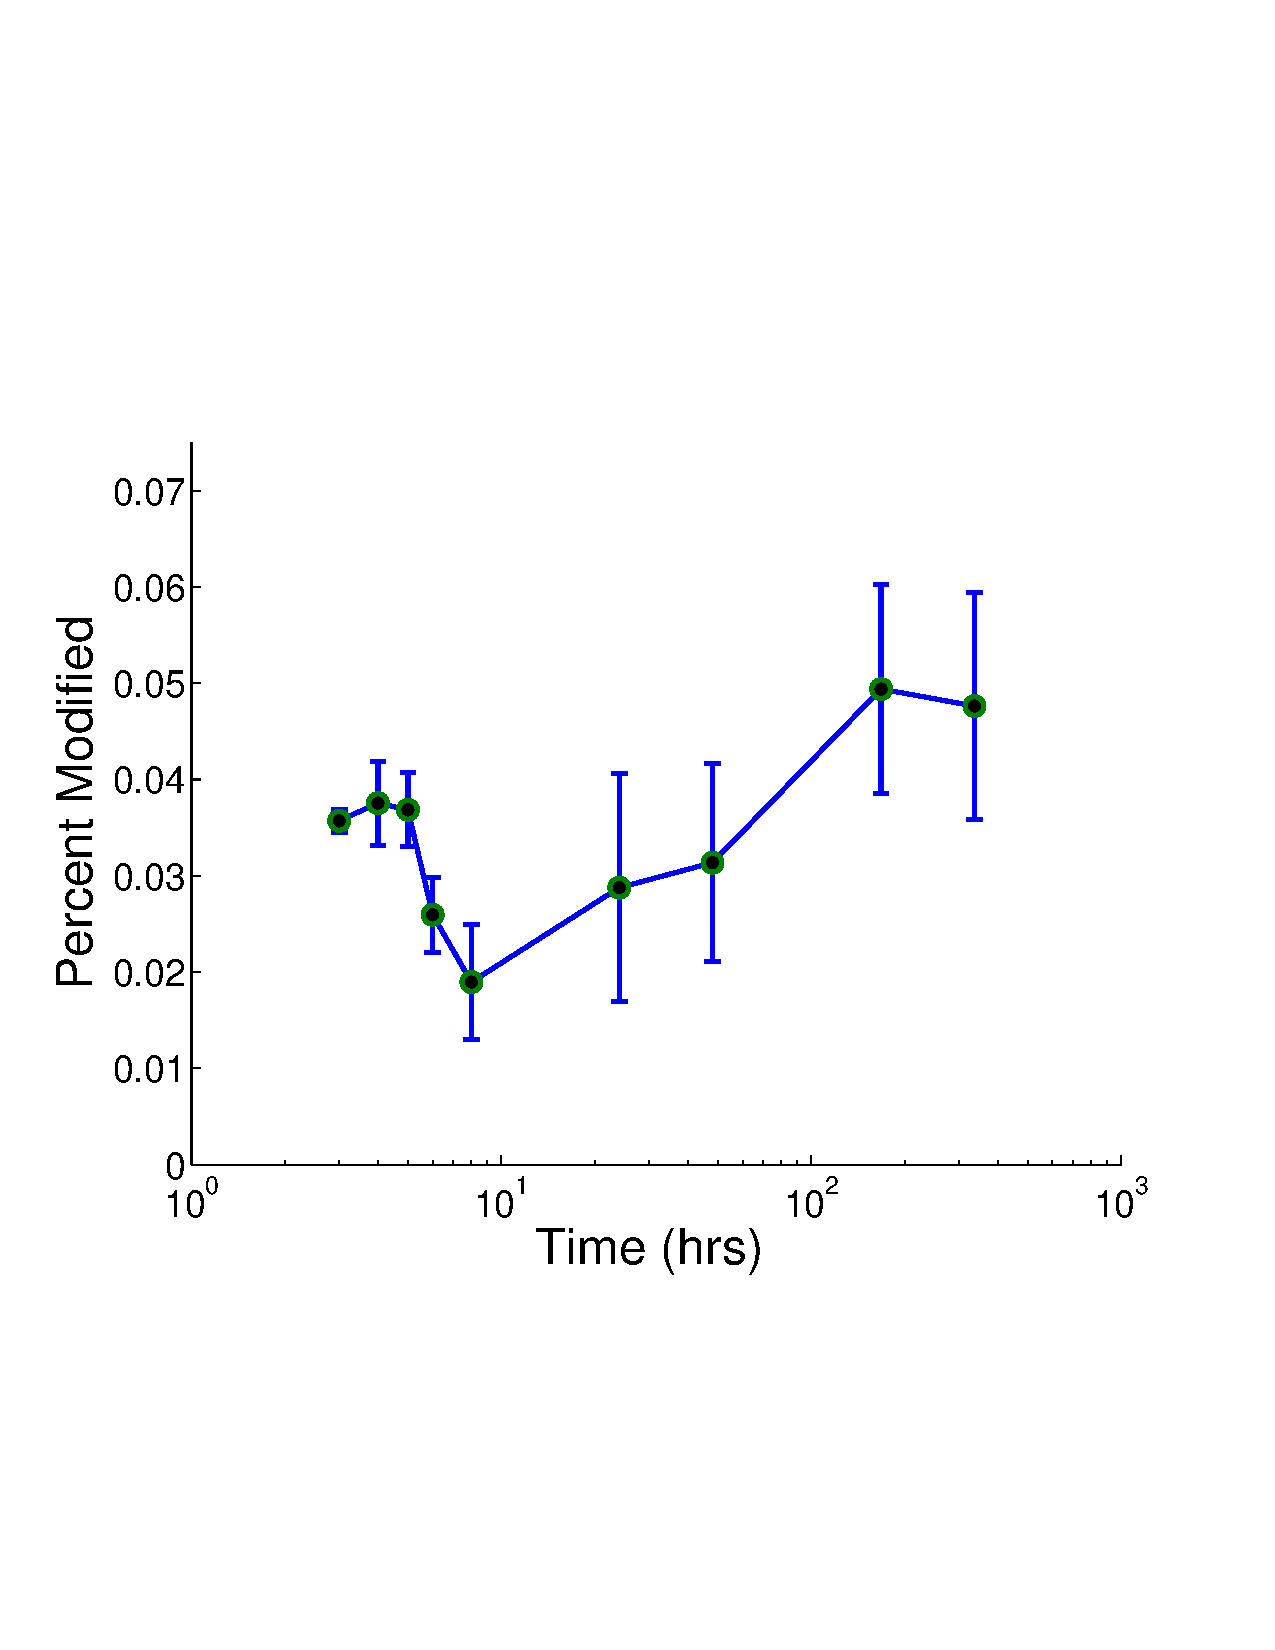
\includegraphics[width=5in]{Figures/Phosphorylations.pdf}}
\caption{\label{fig:carbon_network}\textbf{Predictive .} Reactions .}
\end{figure}


\clearpage
\begin{figure}[p]
\centerline{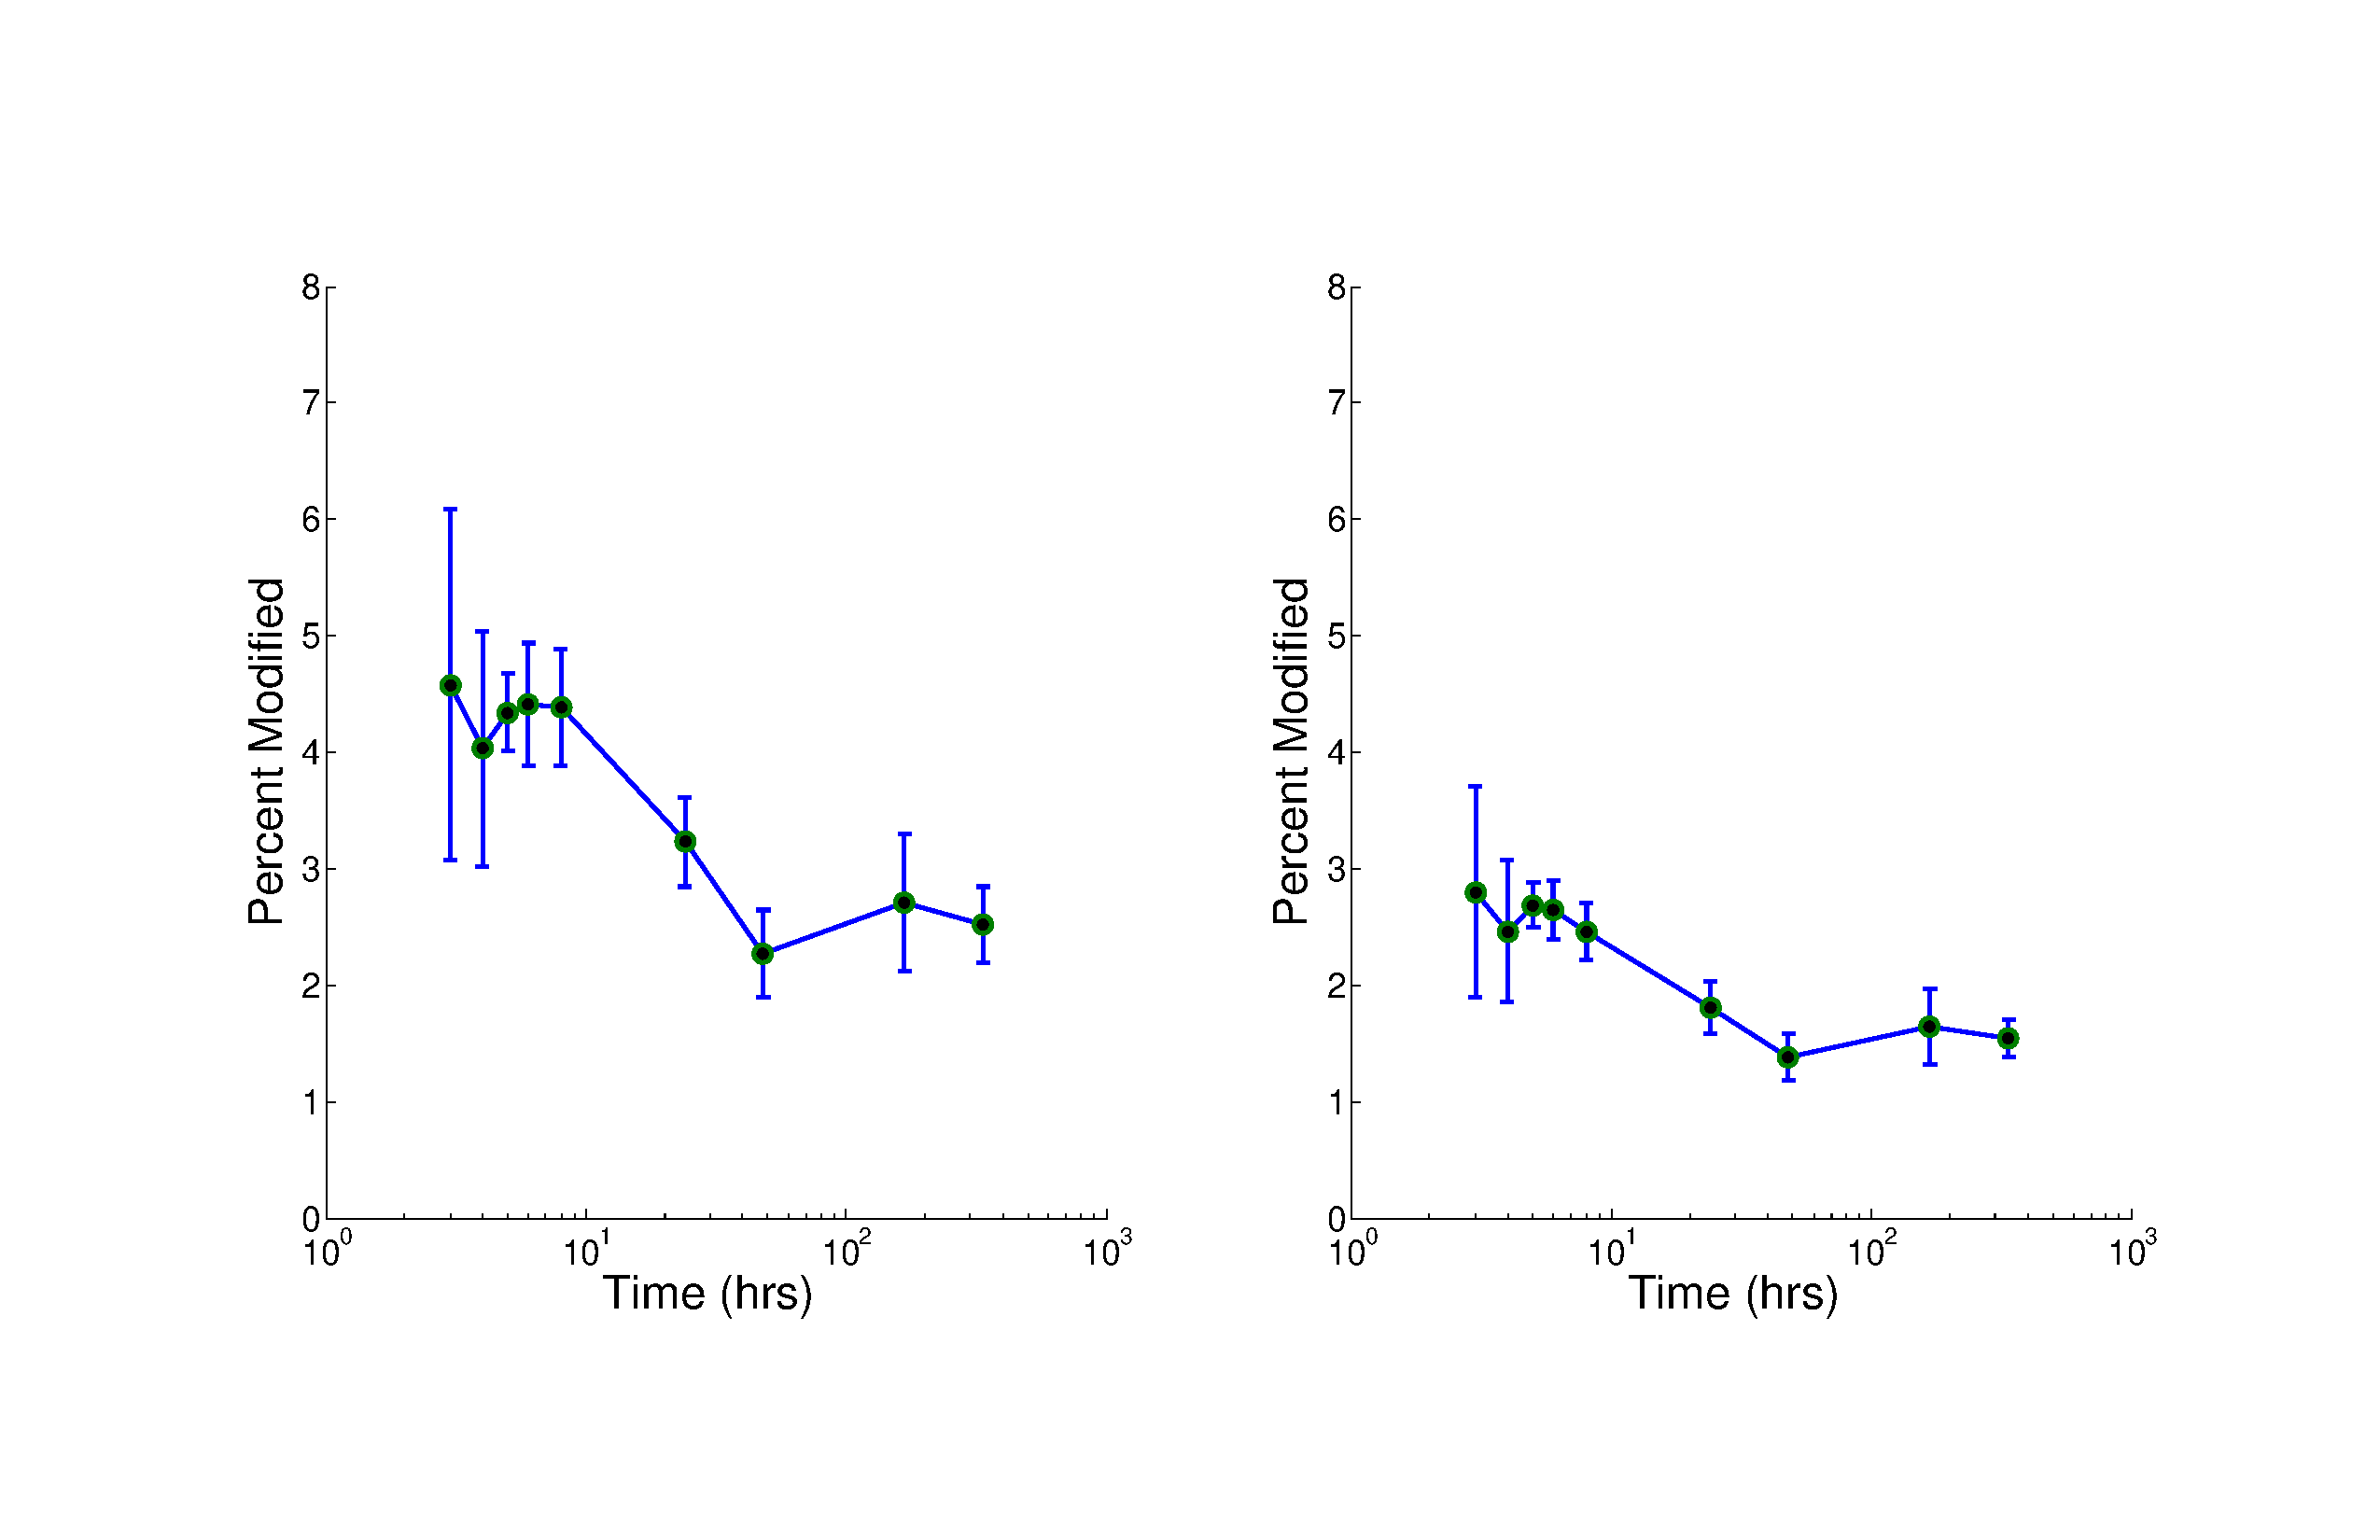
\includegraphics[width=8in]{Figures/Oxidations.pdf}}
\caption{\label{fig:nitrogen_network}\textbf{Predictive .} Reactions .}
\end{figure}

\clearpage
\begin{figure}[p]
\centerline{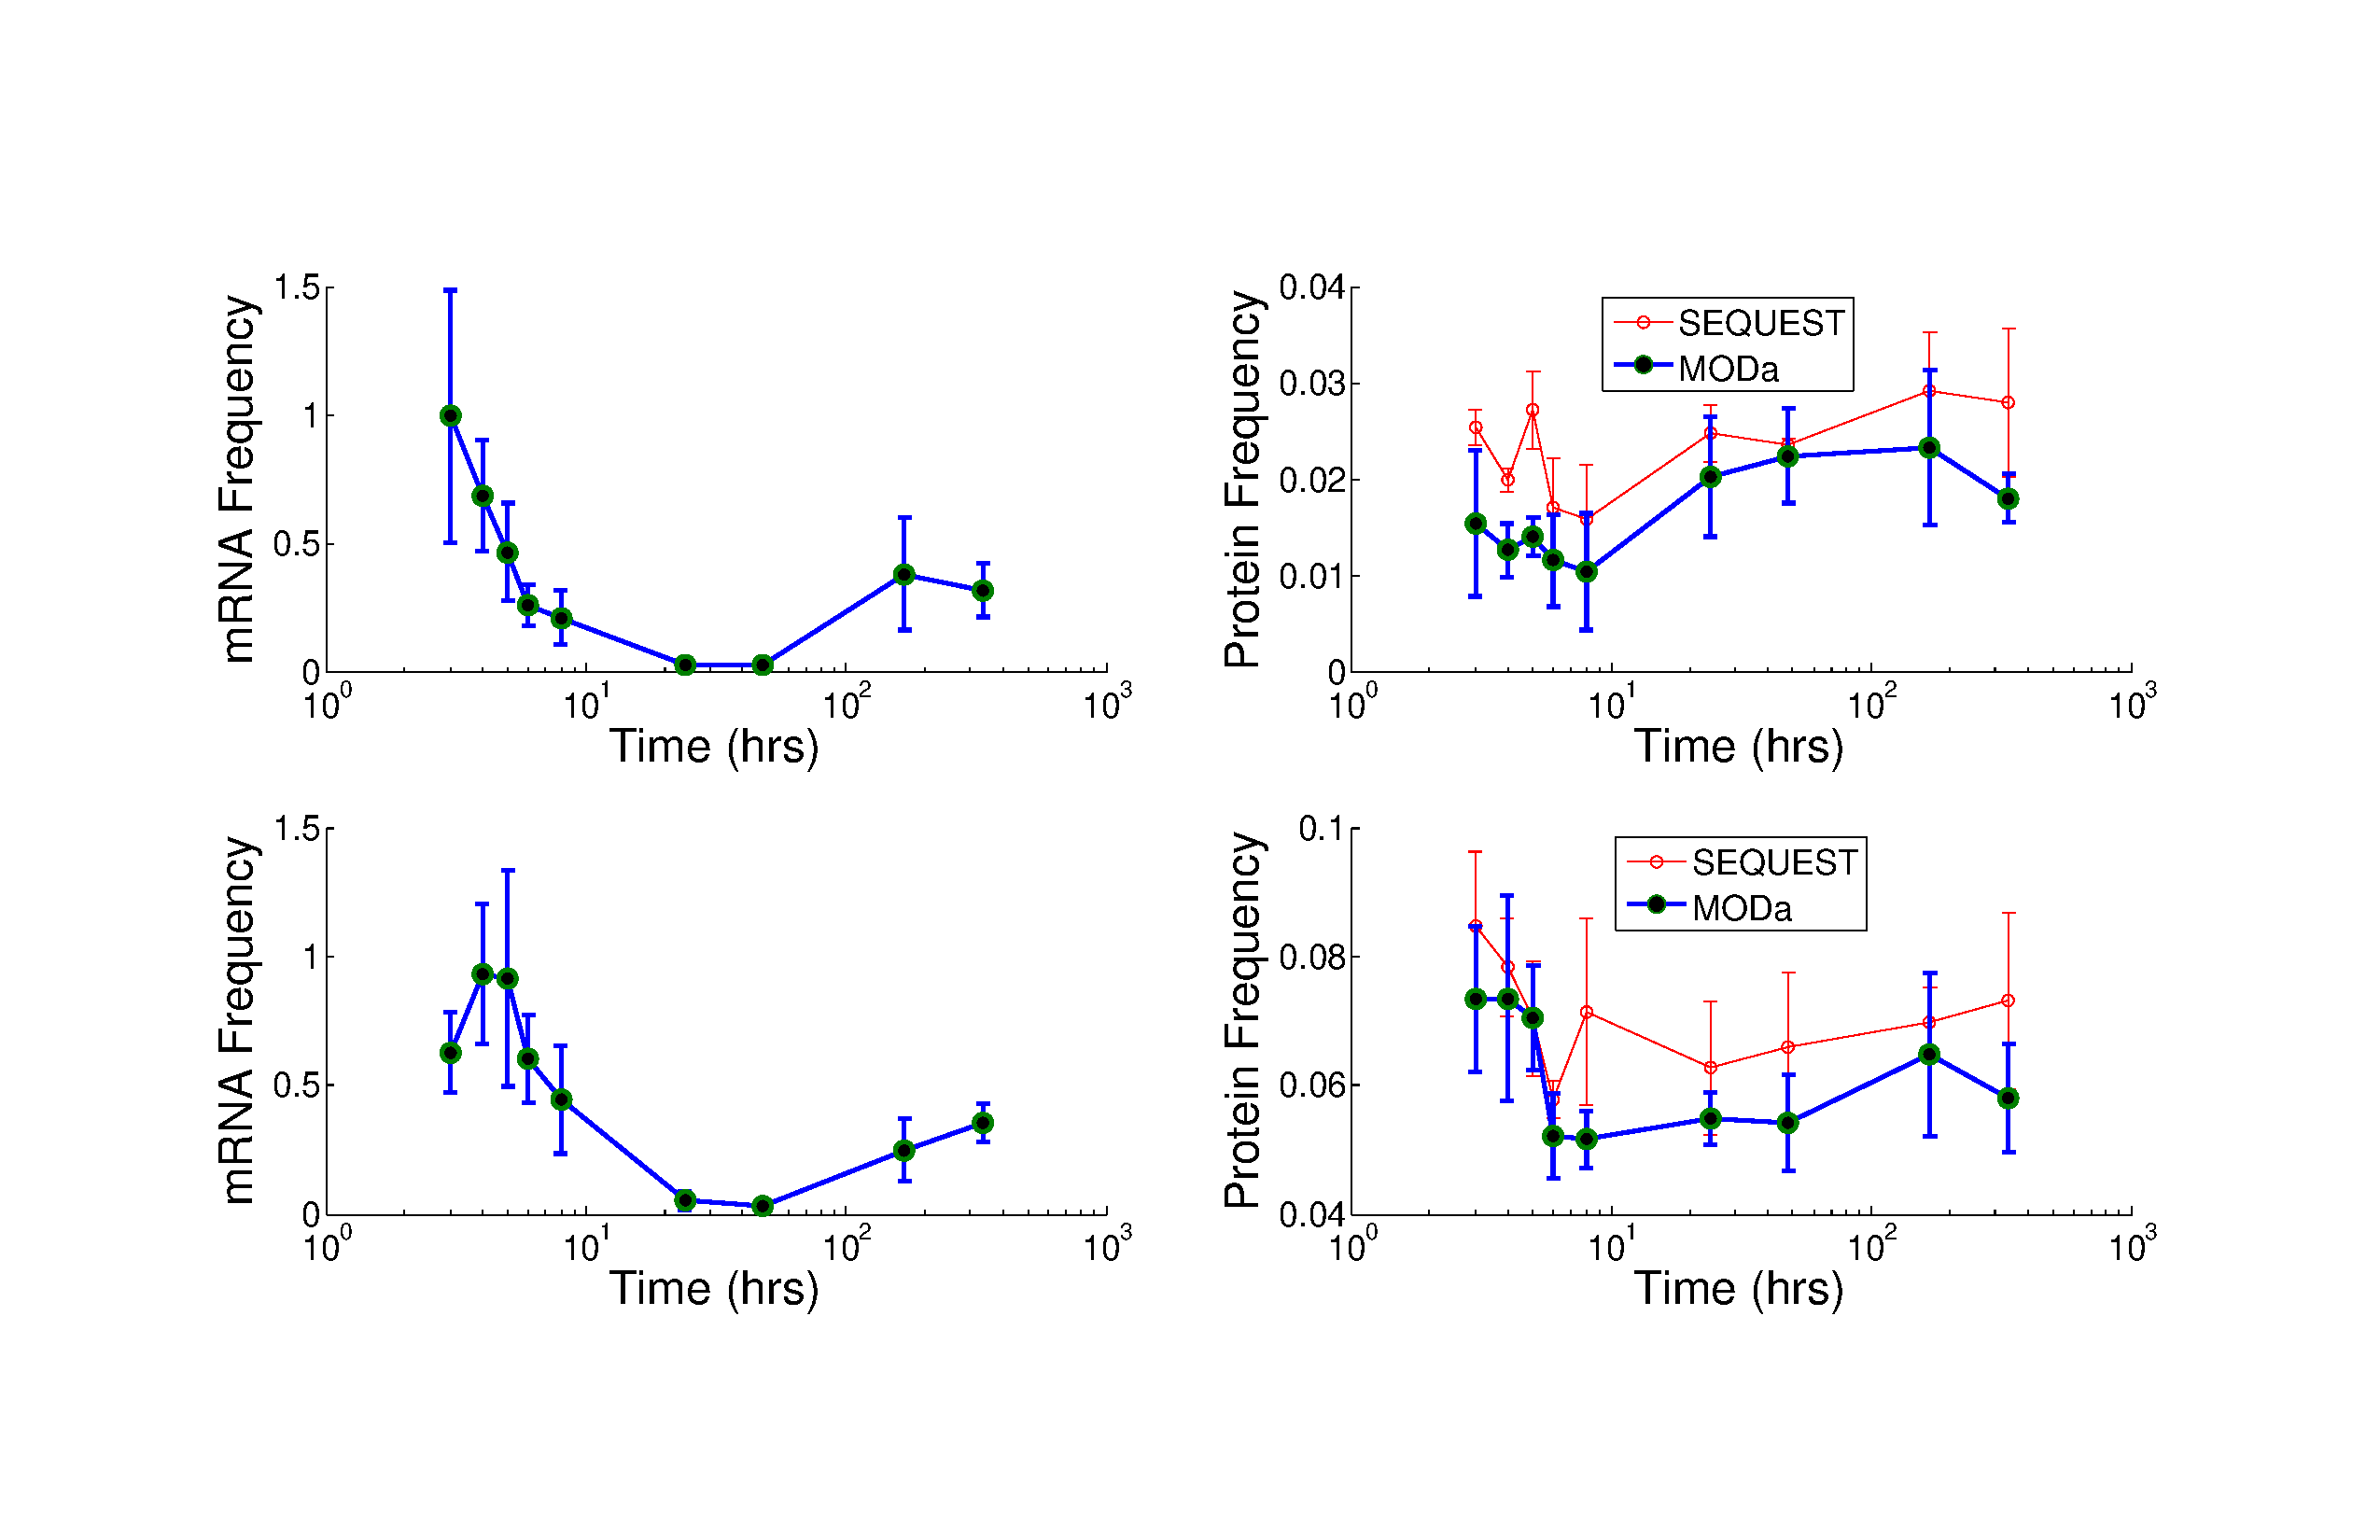
\includegraphics[width=8in]{Figures/MsrAB_mRNA_protein.pdf}}
\caption{\label{fig:nitrogen_network}\textbf{Predictive .} Reactions .}
\end{figure}

\bigskip
\section*{Supplementary Figures}
\clearpage
\centerline{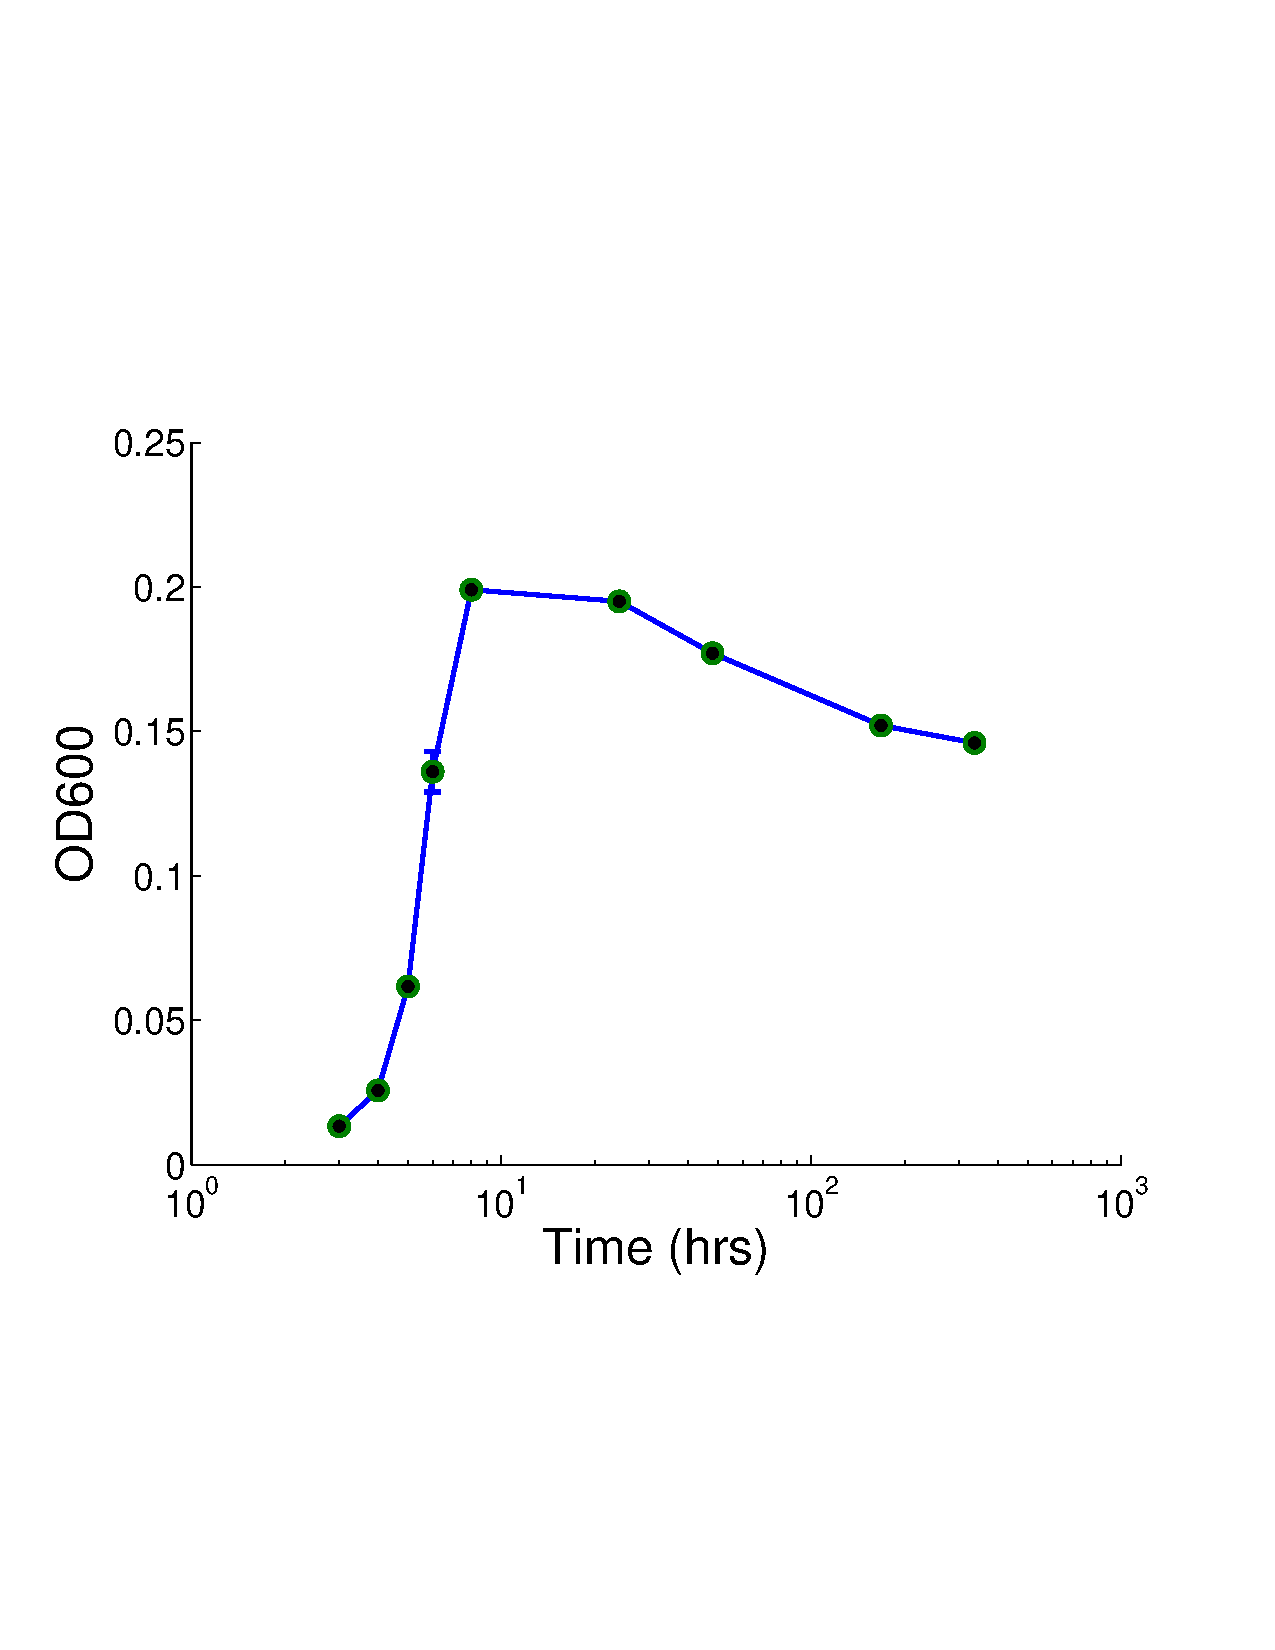
\includegraphics[width=5in]{Figures/PTM_Modified.pdf}}
\customlabel{fig:GrowthCurve}{S1}
\textbf{Figure S1: Scatter .} We .

\clearpage
\centerline{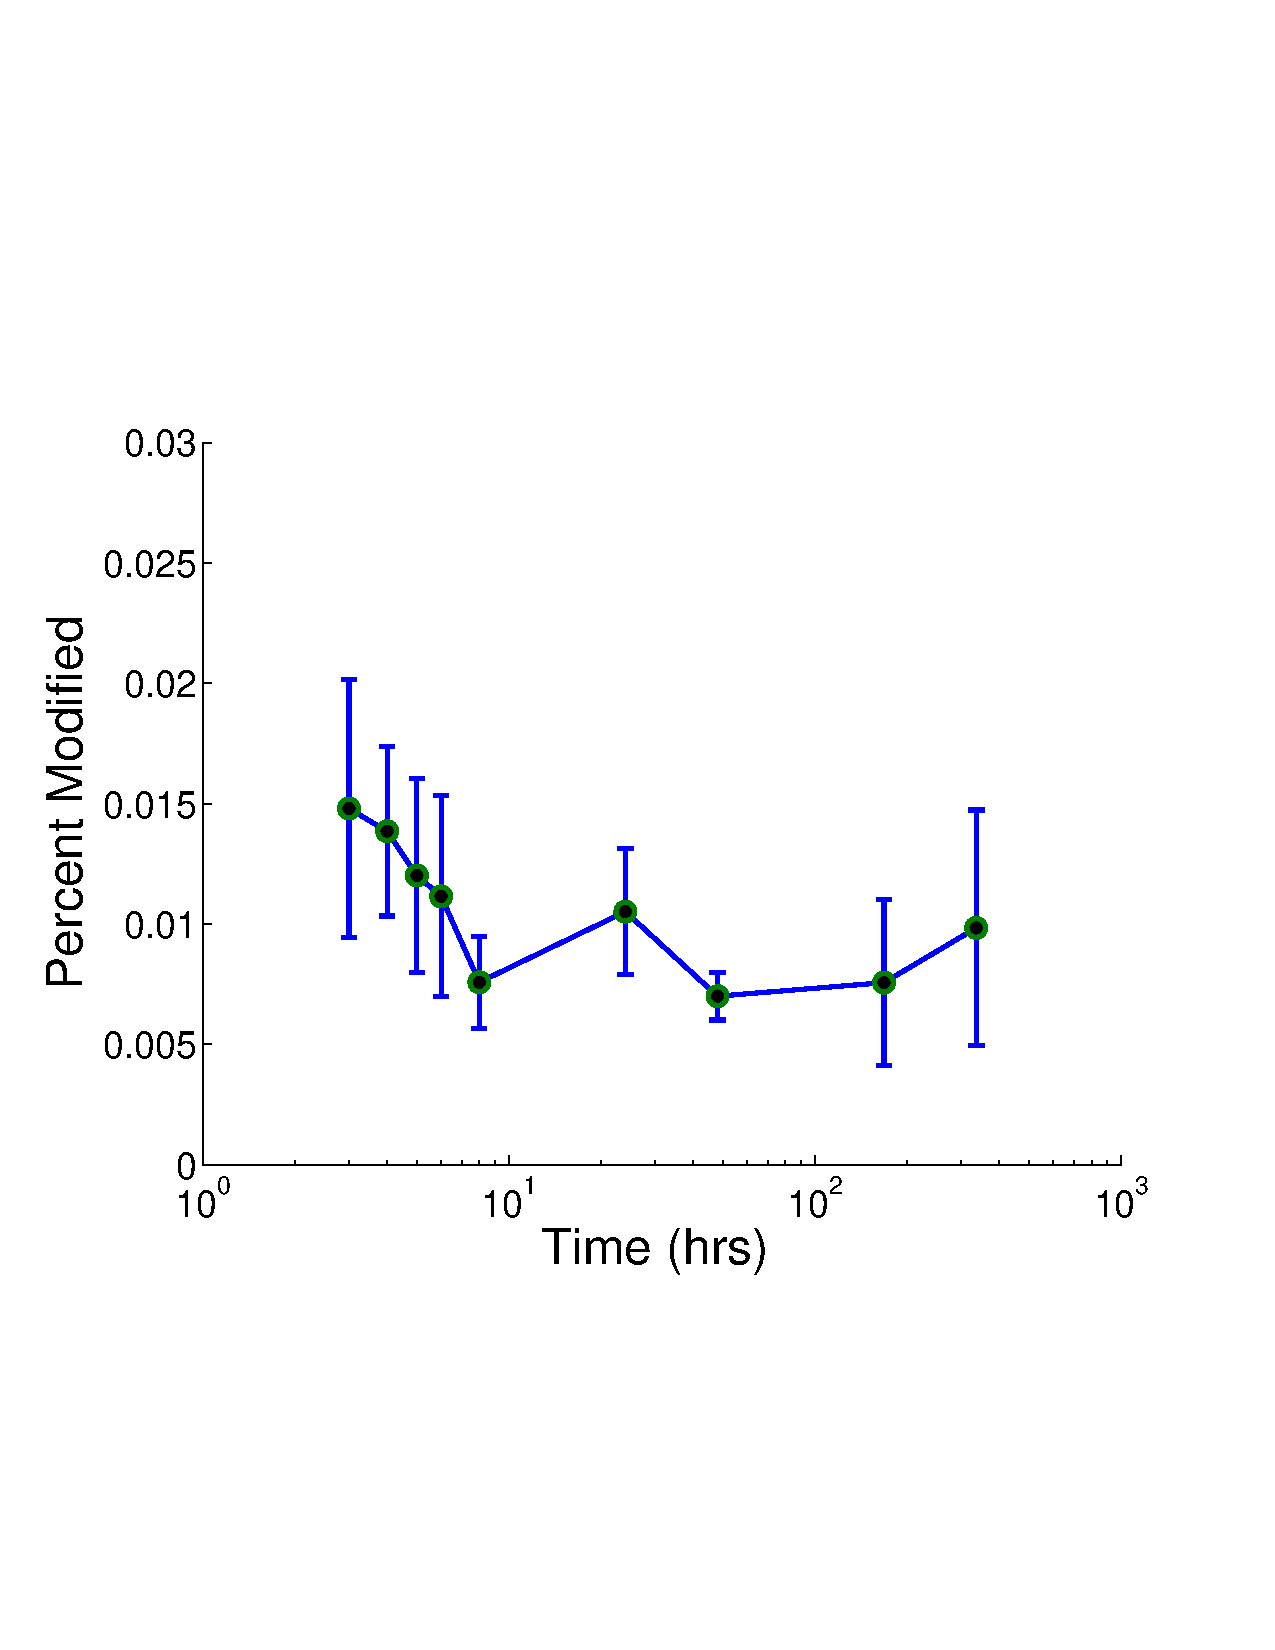
\includegraphics[width=5in]{Figures/Nitrosylations.pdf}}
\customlabel{fig:NitrosylationFig}{S2}
\textbf{Figure S2: Scatter .} We .

\clearpage
\centerline{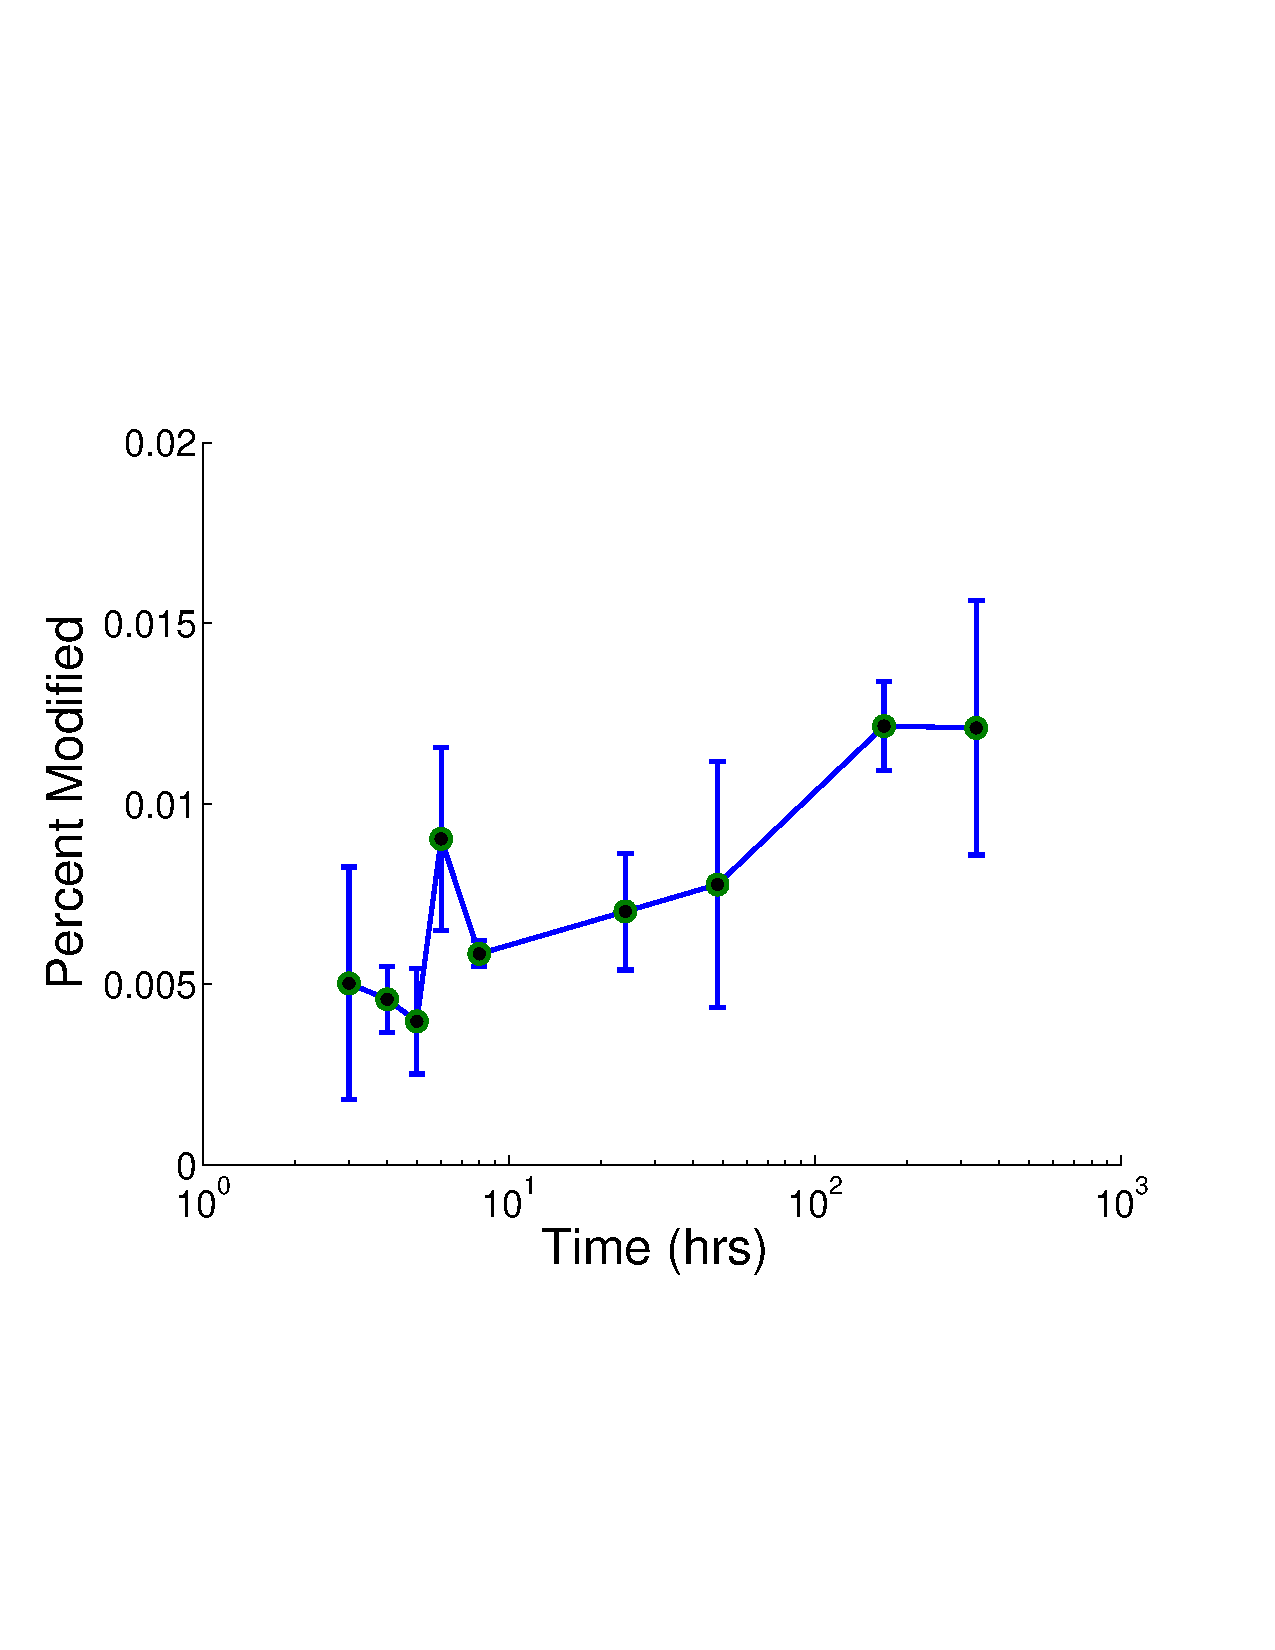
\includegraphics[width=5in]{Figures/Carboxylations.pdf}}
\customlabel{fig:CarboxylationFig}{S3}
\textbf{Figure S3: Scatter .} We .

\clearpage
\centerline{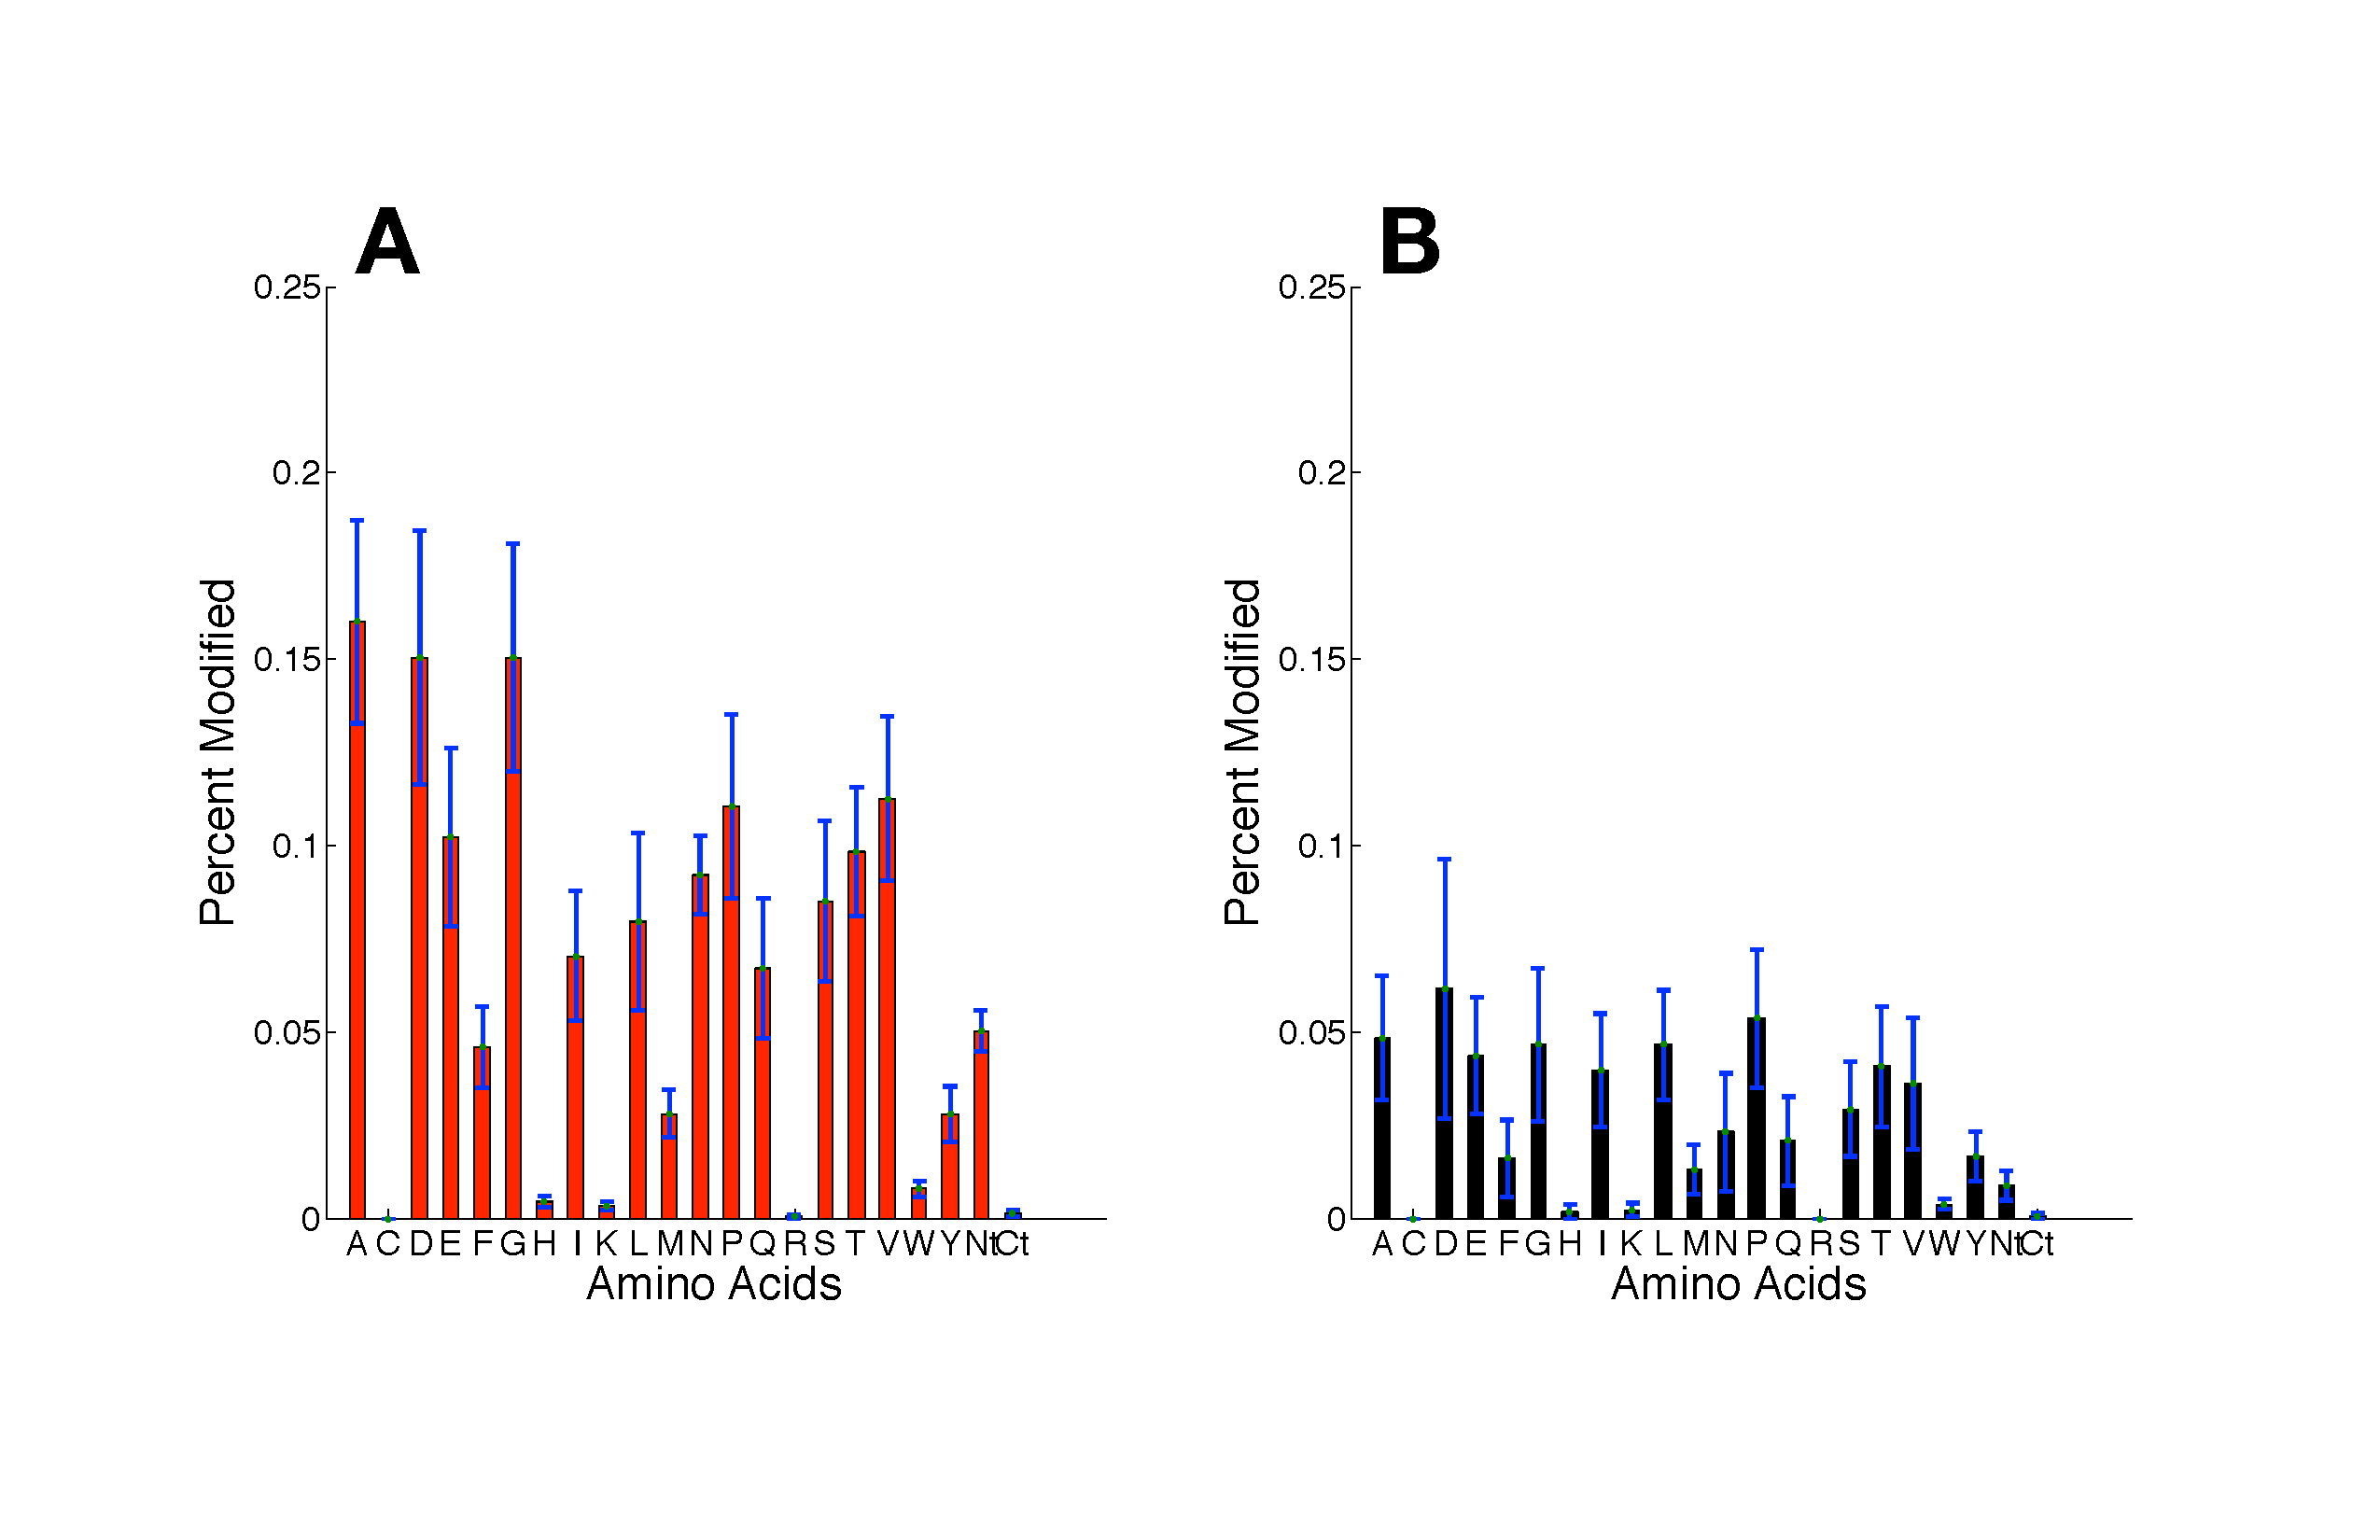
\includegraphics[width=8in]{Figures/NaKAdducts.pdf}}
\customlabel{fig:CarboxylationFig}{S4}
\textbf{Figure S4: Scatter .} We .
%\section*{Supplementary Tables}
%\customlabel{tab:predictive_carbon_sources}{S1}
%\textbf{Table S1: .} These .
%\bigskip

%\noindent File: \texttt{SupportingInfo/CarbonSources.xlsx}\\
%Available in github repository \texttt{https://github.com/clauswilke/Ecoli\_FBA\_input\_prediction}

%\bigskip
%\customlabel{tab:predictive_nitrogen_sources}{S2}
%\noindent \textbf{Table S2: .} These .
%\bigskip

%\noindent File: \texttt{SupportingInfo/NitrogenSources.xlsx}\\
%Available in github repository \texttt{https://github.com/clauswilke/Ecoli\_FBA\_input\_prediction}

\end{document}
